\documentclass{llncs}
 
%% 
% Tasks:
% Ante:
% - SOTA RS and Pervasive 
% Matija:
% - read procedure
% - lifestyle research 
% Marko: 
% - Ang, overall comments

\usepackage[english]{babel}
\usepackage{graphicx}
\usepackage[utf8]{inputenc}
\usepackage{booktabs}
\usepackage{url}

 \def\b{{\beta}}
 \def\gS{{\mbox{gS}}}
 \def\gC{{\mbox{gC}}}
 \def\Id{{\mbox{Id}}}

\begin{document}
\frontmatter  
\addtocmark{Contextual personalization}
\mainmatter 

\title{Theory of planned behavior in user modeling: motivation, procedure and applicational example}

\titlerunning{TPB in user modeling}  
\author{Andrej Košir$^1$ \and Ante Odić$^2$ \and Marko Tkalčič$^3$ \and Matija Svetina$^4$}

\authorrunning{Andrej Košir et. al.}
\tocauthor{Andrej Košir,  Ante Odić, Marko Tkalčič, Matija Svetina}

\institute{University of Ljubljana, Faculty of electrical engineering\\
Tržaška 25, 1000 Ljubljana, Slovenia\\
\email{andrej.kosir@fe.uni-lj.si},
\and
OutFit 7 (Slovenian subsidiary Ekipa2 d.o.o.), \\
Ameriška 8, 1000 Ljubljana, Slovenia \\
\email{ante.odic@outfit7.com},
\and
Johannes Kepler University\\
Strase x, Linz, Austria\\
\email{marko.tkalcic@jku.at}
\and
University of Ljubljana, Faculty of arts\\
Tržaška 2, 1000 Ljubljana, Slovenia\\
\email{andrej.kosir@fe.uni-lj.si}}
  
\maketitle            

\begin{abstract}
The aim of this study was to investigate the use and the potential of the psychological theory of human behavior modeling, called the theory of planned behavior (TPB), in a user modeling domain. We performed a user experiment involving a well studied problem of user modeling: recommender system (RS) for movies. As a part of the TPB, a survey to estimate behavioral, normative and control beliefs regarding movie selection was designed. Using participants’ responses, Ajzen model for movie genres was built and evaluated. Existing public dataset for
context-aware movie recommendation CoMoDa was used to evaluate the proposed method. Results had shown that the TPB approach lead to an accurate prediction of selected movie genres. Among others, the potential
applications of TPB in recommender systems and what is the architecture of such RS were addressed. Questions of what are potential applications of TPB in user modeling domain and what are limitations and drawbacks of it were discussed. 
\keywords{Theory of planned behavior, Ajzen model, Recommender system}
\end{abstract}

\section{Introduction}\label{Sec_Intro} 

User modeling and user adaptation techniques have received much attention in recent decades as the way how to tackle the problem of human computer interaction in broad range of communication services. Recommender systems as a part of this user modeling are today a part of most services that involve content or service selection made by end users. A tremendous amount of academic, industrial research and development was dedicated to develop more efficient user modeling techniques. Many user adaptation tasks can be seen as a problem of effective recommendation of predefined set of entities. Several different directions of algorithm are under development due to the fact that effective user adaptation is very much dependent on the domain of recommendations. However, several drawbacks of existing user modeling techniques are only partially solved such as the problem intrusive end user data acquisition, end user privacy protection, the problem of diversity of RS, etc.

One direction of addressing these issues is to predict end user behavior while he is interacting with the service and utilize such prediction in user adaptation. Human behavior modeling is an intensive research field in psychology for several decades \cite{Martin200703}. The theory of planned behavior \cite{AjzenWebPage} is particularly appealing in user modeling and adaptation for several reasons. First, the behavior model it assumes is relatively easily interpreted in several domains in the way that the available adaptation domain knowledge can be utilized. Second, the procedure of building the Ajzen model for a given domain is a well defined procedure (we present it in Sec. \ref{Sec_AzenProc}). Third, the prediction model is not predefined but can be selected according to the domain knowledge. Fourth, there is a large amount of modeling cases providing rich past experiences resulting in effective modeling guidelines.  

We present the procedure of Ajzen model building including how to select predefined behaviors and demonstrate the model on a real users dataset. We discuss the potential of this type of psychological modeling of human behavior in user adaptation procedures. Discussion also addresses constrains and issues of further development in regard to implementation of TPB into RS.


\subsection{Related work}\label{SubSec_RelatedWork}

The usual reasoning in user modeling procedures is to build a model of a user $u$ according to his past treatment of domain items $h$. These items are multimedia content items, tourist destinations, selected food etc. These models are build according user history related to this items (content based), according to the history users $v$ of similar to the users $u$ (collaborative based) or the combination of these two approaches (hybrid). The involved machine learning algorithms are designed to optimize the selected performance measure. No underlying mechanisms that governs the user's interaction with the system are typically taken into account. For example, the Netflix price wining algorithm Matrix Factorization (MF) \cite{koren2009matrix} has no model of users or items that is based on users or items features (metadata). 

\subsubsection{Recommender systems}\label{SubSubSec_RS}

The main goal of RSs is to predict the ratings for the items that the user has not consumed yet. Based on the predicted ratings, the suitable items (those with high predicted ratings) are selected and provided as the recommendations. Content-based (\textbf{CB}) recommender systems \cite{pazzani2007content}  analyse the items’ descriptions in order to learn the user's preference for specific types of items. The prediction for the unseen item is based on the ratings for similar items by the same user. There are many limitations of CB systems: the system depends on the metadata which has to be explicitly associated with each item; overspecialisation due to the item-similarity paradigm; the users are not given serendipitous recommendations and the user is held in the so-called "filter bubble" \cite{pariser2011filter}. In Collaborative Filtering (\textbf{CF}) strategies the prediction for the unseen item is based on the opinion from users with similar tastes \cite{resnick1994grouplens}. This approach ignores the items' metadata so cross-domain recommendations are possible (e.g., books, movies, music, etc.) by employing cross-domain techniques \cite{fernandez2012cross}. After the Netflix prize competition \cite{bennett2007netflix}, matrix factorization has become a popular CF technique \cite{Koren2008factorization,koren2009matrix}. When a substantial amount of ratings are present in the system, these techniques tend to outperform other approaches. However, according to \cite{balabanovic1997fab}, for the user whose tastes are unusual compared to the population, the similarity to other users will be poor, hence resulting in poor recommendations for such a user. Knowledge-Based (\textbf{KB}) systems use knowledge from the domain expert in order to prepare meaningful recommendations \cite{schafer1999recommender}. However, pure KB systems are not popular and widely used, since they are expensive due to the required input from the domain expert. In order to overcome the different problems with the CF and CB strategies, they are sometimes combined into the Hybrid RS \cite{burke2007hybrid}. Furthermore, some context-aware techniques actually fall into the hybrid-system strategies, since the basic rating prediction can be made in one way and later adapted by the contextualization, e.g., post-filtering contextualization \cite{Adomavicius2011}. 

This kind of model construction has a number of constrains. One way to address these issues is to gain additional knowledge in regard to underlaying mechanisms of user's interaction with the system. For example, a design of effective pervasive systems typically requires a deep domain knowledge including the understanding of parameters and mechanisms of users behavior practices. One such model is Lazy User Theory \cite{Tetard2009}. Authors developed a theory that a user will most often choose the solution that will fulfill her information needs with the least effort. Such assumption allows us to explain selection factors using multivariate statistics but it also assumes that a user has a clear defined goal in while seeking information. However, it seems this simple and strong hypothesis is not valid in many situations of user interaction with information systems due to the fact that modern users uses these systems with no specific goal. A different theory, TPB seems more promissing in this context. The theory and the rationals for applying it in the RS context are provided below.  


\subsubsection{Theory of planned behavior (TPB)}\label{SubSubSec_TPB} A pioneer work on theory of planned was carried out by Icek Ajzen \cite{Ajzen1991} and model suggested by TPB is usually called Ajzen model. 

Ajzen model was introduced as a complete model for explaining human behavior and is based on a large number of behavior studies. According to TPB, human behaviors are influenced by attitudes towards the behavior, by subjective norms regarding the behavior and perceived behavior control \cite{Ajzen1991}, see Fig. \ref{Fig_TPB}. Behavior is domain specific; in this study we selected the behavior as a selection of a movie with a given genre. Attitudes are beliefs that one person has about the outcomes of the behavior (seeing the selecting movie) and are divided into cognitive, emotional and behavioral. Subjective norms are related to beliefs about the expectations of others and the wish to comply them. Behavior control relates to the ability one can perform the preselected behavior and this directly affect the decision about the behavior. 

 \begin{figure}[h!]
 \begin{center}
   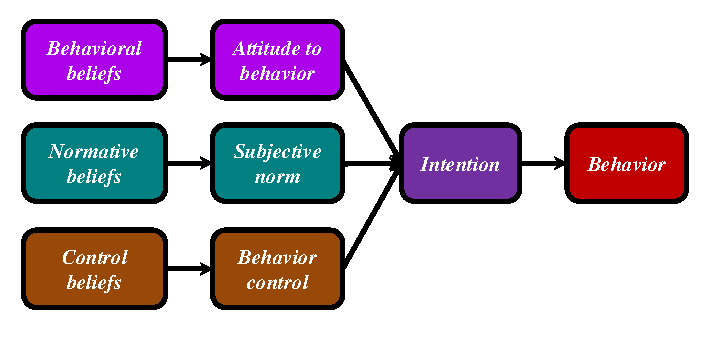
\includegraphics[width=9cm]{TpbScheme.pdf}
   \caption[Fig_TPB]{A diagram of Theory of planned behavior \cite{AjzenWebPage}.}
   \label{Fig_TPB}
 \end{center}
 \end{figure}
 
There are several areas where human decision making is of key importance exhaustively studied by TPB models such as outdoor recreation activities \cite{Daigle2002}, decisions related to high school studies  \cite{Davis2002}, public transportations habits \cite{Bamberg2003}, health related behavior \cite{Ajzen2007},  consumer attitudes and behavior \cite{Ajzen2008},  employers' hiring intentions \cite{Fraser2010} and job satisfaction \cite{IcekAjzen2011}, adoption of wireless sensor network service in households \cite{Lin2011}, factors Influencing the intention to watch online video advertising \cite{Lee2011} and mobile phone usage while car driving \cite{Walsh2008},\cite{Zhou2012}. 

The common goal of these studies is not only to be able to predict human decision but also to understand the underlying mechanism of these decisions. These explanations are then used to create a new theory or to modify existing ones in order to provide a further insights of the targeted domain. 

Extensive tutorials of how to effectively build and apply models of TPB in practice are available online \cite{AjzenWebPage}.  A guide for conducting statistical analyses in a reasoned action context is given in \cite{Bleakley2012}. Further research directions related to TPB and Ajzen model are surveyed in \cite{Jaccard2012}.




\subsection{Problem statement}\label{SubSec_}

The goal of this papers is to provide a rational for using the Theory of planned behavior (TPB) in user modeling applications. We present the background of the TPB and outline the procedures for the acquisition of the TPB parameters. As a proof-of-concept we present the results of an experiment where we used in TPB model in recommender system for movies. 


%In this research we address the problem of prediction of complex groups of items such as movie genres. We believe the underlying mechanisms of selection of such groups of items is more complex than the selection of individual item. Consequently it requires refined modeling of user decision making. When user selecting an item, end user undergoes several decision steps along different paths according to his motivation, past experience etc. To model these procedures we considered several user decision making models and select theory of planned behaviour known as Ajzen model \cite{Ajzen1991}.  


\section{The procedure of model building}\label{Sec_AzenProc}

We list the below given procedure of TPB model building to collect the most relevant guidelines and potential errors for the UM community. There are two reasons why a crucial step of the model building is the selection (definition) of behaviors. The first one is the fact that the quality of the model is mainly limited by the selection of behaviors, details are given at step 1. below. The next one is that selected behaviors also defines the role of the modeling itself. These roles can vary from predicting groups of items to the explanation of the specific aspect of the decision making process. We elevate on this in section \ref{Sec_Disc}.

\begin{enumerate}
 \item {\it Define a set of behaviors.} As indicated above, this is the most important step of the whole modeling task. Prior to it the reason why we apply the TPB must be clarified. In this paper given example the reason was to further understand mechanisms of movie selection. Preliminary results showed that there are high variabilities among users regarding genres of movies they select. So we conclude that understanding reasons for these variabilities would provide the insight that we can utilize to improve the accuracy of user model in move recommender. If we defined behaviors as selection content item (each movie was associated to one behavior) we would gain no explanation. Besides, the model quality would be very low due to the lack of separability of behaviors. This observation leads to the second guideline which is related to the quality of model fitting. The behaviors are required to be discriminable by the reasonable user data. This means that the survey (see step 2.) used to acquired user data is feasible, that is short enough and clear enough. Also, it is clear that two behaviors that are the same in most of end user situations can not be discriminable. For example, if two genres are both either present either not not present in almost all movies selected by users, these associated behaviors can not be discriminable. To summarize, the behavior definition should relay on a end user data analysis and on the clear goal of the modeling itself.  
 \item {\it TPB questionnaire construction.} The next step is to design a questionnaire for end users in order to estimate parameters of the model. It must meet the requirements set by TPB. We group them into three groups regarding Behavioral beliefs (about consequences of the behavior), normative beliefs (about expectations of others) and control beliefs (about factors that affect the performance of the behavior). Therefore, this construction requires deep domain knowledge of the selected behaviors. The base of all questions are the defined behaviors (see step 1.). The next issue addressed is the specification of end user population. Five to six questions are then formulated to assess each of the constructs (attitude, norms, control and intention). For each question, the type of answers is selected. As usual, the next phase is administering a pilot questionnaire, its evaluation on a small population following by a standard questionnaire construction.
 \item {\it Select and build the prediction model.} According to the constructed questionnaire and a set of predefined behaviors, a prediction model is selected. First, the criteria variable indicating the true behavior is constructed. In our example of movie genre selection, for the first the criteria variable is computed from the past movie selection of the targeted end users (see Sub. \ref{SubSec_CritConstr}).  For the second model, the criteria variable is the simply genre indicator of the most likely selected genre by this end user. Next, the model itself is selected. Typically, the first option considered is linear regression model if predictor and criteria variables fits the requirements. Options are also linear discriminant analysis, logit regression model, canonical regression, structural equation modeling etc. In general, there is no limitation from the TPB imposed on the model selection. For example, one could apply neuron network to model the relationship among predictor and criteria variables. However, the explanation power of the selected model also matters since the interpretation of the fitted model may provide useful hints for further improvement of user adaptation procedure. 
 \item {\it Interpret the model.} Interpretation of models are based on standard interpretation of selected models. For instance, linear regression model is interpreted according to the sign and magnitude of the estimated normalized model coefficients etc. Again, the main aim of the model is 1) to gain additional insight into the mechanisms behind movies selections, and 2) to improve the performance of RS. 
\end{enumerate}


\section{Materials and Methods}\label{Sec_MatAndMeths}  

In this section, we first explain procedures undertaken to measure behavior; following we explain how and why we used TPB variables for modeling the behavior.   


\subsection{Participants}\label{SubSec_Participants}

In our experiment we had 28 subjects aged between 17 and 38 years old (18 males and 10 females). Each of the subjects filled-in a TPB questionnaire using GDrive forms. Users were selected from contributors of movie ratings in contextual movie dataset CoMoDa \cite{CoMoDa2009}.


\subsection{Instruments}\label{SubSec_Instrum}

The constructed TPB questionnaire consists of 49 questions related to beliefs regarding move selection and consumption according to TPB and is available on-line. The filling time was 10 to 12 minutes. Most of the answers were $5$ level Likert scales Not important - Important (38), some were binary (2) and No - yes (7) and some required free text answer (3). The questionnaire is available upon request to the corresponding author of this paper. 

% -iz vprašanj napovemo vedenje: žanr

\subsection{Construction of criteria}\label{SubSec_CritConstr}

We describe the ground truth user behavior by two criteria variables determined from known users past movie selections and ratings they provided for the dataset CoMoDa \cite{CoMoDa2009}. Each of the rated movie in the dataset has three genres assigned to it.  The first one is genres scores denoted by $\gS(u, g)$ where $u$ is user and $g\in\{\mbox{drama}, \mbox{action}, \mbox{comedy}\}$ is the movie genre. It is defined as a ration between the number of movies selected having genre $g$ and the number of all genre (movie) selections. For example, if a user $u$ has rated $45$ drama movies and provide $91$ ratings to the database, we have $\gS(u, \mbox{drama}) = 45/(3\cdot91)=0.1648$ since every movie selection means a selection of three genres. 

The next criteria variable we introduce is genre membership $\gC(u)$ where $u$. Indexes of genres (also behaviors in our case) are $\Id_{\mbox{\tiny drama}}=1$, $\Id_{\mbox{\tiny action}}=2$ and $\Id_{\mbox{\tiny comedy}}=3$. $\gC(u)$ is defined as the index of users preferred genre for which users expected rating is the highest. These expected scores are computed from users past genre ratings. Here we assume that users has rated mostly movies with genres he prefers since the rating in the dataset are collected for movies the user selected to see by his preference and not by our recommendation. For example, if a user $u$ has rated $45$ drama movies and his average rating for these movies is $3.82$ while average ratings for action and comedy are lower, we set $\gC(u)=\Id_{\mbox{\tiny drama}}=1$.
% - opis odvisno spremenljivke: kaj pomeni 0.7 v rezultatu
% - korelacije med kriterijem in ocenami filmov: yDrama in ratingi
 
\subsection{Construction of predictor variables}\label{SubSec_PredVarConstr} 

To allow the explanation of contributions of the three beliefs (behavioral, normative and control, see Subsec. \ref{SubSubSec_TPB}) of TPB, we decided for the hierarchical model. As depicted at Fig. \ref{Fig_AggregModel}, we fit the following six models:
\begin{enumerate}
 \item Each of three beliefs is regressed to score showing the contribution of each beliefs to the selection of behavior (movie with a given genre). The criteria variable used is $\gS$ and this yields to a nine models. In these models, predictor variables are answers to questions assigns to the modeled belief;
 \item Aggregated model: Prediction of scores of each of three beliefs obtained (previous step) are used as predictor variables model the selected behavior. 
\end{enumerate}
For genre scores $\gS$ we selected multivariate linear regression (MVR) and for genre membership we used linear discriminant analysis. 
According to our understanding of users movie selection mechanisms, factors affecting the decision for each of selected genres may vary. For instance, for selecting drama a main actor may be the most important factor while for selecting actions the movie director   may be the key for the decision. Therefore, we decided to use multivariate models with different slopes, that is for each of the selected behavior we get different regression coefficients. The score of the model is a triple $(s_D, s_A, s_C)$ computed by inserting users answers into MVR models for genres Drama, Action and Comedy, respectively.  


\section{Results}\label{Sec_Results}

As already indicated, the selected behaviors we model are selection of three movie genres drama, action and comedy. In this section we list and briefly explain results of TPB models fitting of user data acquired by the designed questionnaire.  For each of six models fitted and tested (three models from attributes, one from norms and control, and the top level aggregate model) we fitted MVR model (resulting in model coefficients $\beta_k$ and a proportion of explained variances $R^2$) and performed linear discriminant analysis (resulting in discriminant weights $w_k$ and separability $s$ in terms of Fisher discriminant analysis \cite{RencherChristensen201207}). We do not report results for all six models, but only for the cognitive attributes (selected for demonstration how to interpret results) and for the aggregate model which summarizes the whole TPB model. 


\subsection{Selected sub-model: cognitive attitude toward the behavior}\label{SubSec_CogAttr}

This sub-model explains the role and contribution of user's answers to eight questions $Q_1 - Q_8$ regarding cognitive attributes toward the behavior (i.e. the selection of a movie of one of selected genres). At Fig. \ref{Fig_AggregModel} depicting the aggregated model, this sub-model is located on the top of three sub-models explaining user's attribute toward the behavior.

The proportion of explained variance for the cognitive attitude toward the behavior is $R^2=0.48$. This high value allows us to interpret beta coefficients of the model and determined the relative importance of cognitive attitude in the overall mode as discussed  in Subsec. \ref{SubSec_AggregateModel}.

A normalized MVR model coefficients are listed at Tab. \ref{Tab_attitudeCog_MvRegress}. Coefficient $\b_0$ 
represents the offset of the resulting model, coefficients $\b_k$, $1\leq k \leq 8$ corresponds to questions $Q_k$. Significant $\b$ coefficients are marked with $^*$. 
\begin{table}[!h]
  \centering
   \begin{tabular}{|l|c|c|c|c|c|c|c|c|c|}
\hline
\textbf{Genre} &\textbf{$\beta_{0}$}&\textbf{$\beta_{1}$}&\textbf{$\beta_{2}$}&\textbf{$\beta_{3}$}&\textbf{$\beta_{4}$}&\textbf{$\beta_{5}$}&\textbf{$\beta_{6}$}&\textbf{$\beta_{7}$}&\textbf{$\beta_{8}$}\\\hline\hline
\textbf{Drama}&0.32&0.02&-0.03&-0.01&-0.02&0.01&0.00&-0.01&0.00\\\hline
\textbf{Action}&3.43&0.09&-0.11$^*$&0.10$^*$&0.05&-0.08&0.13$^*$&-0.02&-0.02\\\hline
\textbf{Comedy}&3.69&0.48$^*$&-0.34$^*$&0.05&0.07&-0.04&-0.12$^*$&-0.11$^*$&0.06\\\hline
\end{tabular}

  \caption{MVR coefficients of cognitive attitude toward the behavior predictors, $R^2 = 0.48$.}
  \label{Tab_attitudeCog_MvRegress}
\end{table}
We observe that no coefficient that models the genre Drama is significant and therefore no conclusion can be made here. This is most probably due to the relatively low sample size used to fit the model. Regarding the genre Action, coefficients representing $Q_2=${\it How important for you is the story in the movie?}, $Q_3=${\it How important for you is the movie's genre?} and $Q_6=${\it How important for you are the special effects?} are significant. Since $\b_2$ is negative, users that does not care much about the story of the movie are more likely to select drama. Positive coefficients $\b_3$ and $\b_6$ show that users that care about genre and special effects are more likely to select drama. 

In the same way we interpret the selection of Comedy movies. Large positive coefficient $\b_1=0.48$ representing $Q_1=${\it How important for you is the main actor of the movie?} indicates that main actor is the most important factor in selecting comedy while $\b_2$ representing $Q_1=${\it How important for you is the story in the movie?} indicates that the story has very little relevance in selecting the comedy. Coefficients $\b_6=-0.12$ and $\b_7$ representing questions $Q_6=${\it How important for you are the special effects?} and $Q_7=${\it How important is an attractive trailer?}, respectively, indicates the low relevance of the special effects and of the trailer in comedy selection. 

We analyzed the separability of genre selection behaviors by LDA. The Fisher separability of the cognitive attitude toward the behavior is $s = 0.81$ what is a moderate separability. The LDA coefficients separating given pairs of genres are listed in Tab. \ref{Tab_attitudeCog_LDA}. Significant coefficients are labeled by $^*$. A significant contribution to the separation of genres Drama and Action are obtained from $Q_3$ and $Q_6$ etc. 

\begin{table}[!h]
  \centering
   \begin{tabular}{|l|c|c|c|c|c|c|c|c|}
\hline
\textbf{Genre pair}&\textbf{$w_{1}$}&\textbf{$w_{2}$}&\textbf{$w_{3}$}&\textbf{$w_{4}$}&\textbf{$w_{5}$}&\textbf{$w_{6}$}&\textbf{$w_{7}$}&\textbf{$w_{8}$}\\\hline\hline
\textbf{Drama/Action}&-0.87&-0.82&-3.26$^*$&-0.66&-0.42&-3.54$^*$&1.68&-0.01\\\hline
\textbf{Drama/Comedy}&-5.67$^*$&-0.49&0.94&0.09&-1.48&-1.23&1.19&-1.56\\\hline
\textbf{Action/Comedy}&-4.80$^*$&0.32&4.19$^*$&0.75&-1.07&2.31&-0.49&-1.55\\\hline
\end{tabular}

  \caption{Linear discriminant coefficients of cognitive attitude toward the behavior predictors.}
  \label{Tab_attitudeCog_LDA}
\end{table}

To summarize the interpretation, questions and underlying decision factors that are relevant in both models (MVR and LDA) are regarded as the most important. These are $Q_1$, $Q_3$ and $Q_6$. The question $Q_1$ is the most important one since it is involved in discriminant function with high magnitudes. The behavior of selecting Drama is not modeled well (no sig. MVR coefficient) while the behavior of selecting genre comedy is model well. 

\subsection{Aggregated TPB model}\label{SubSec_AggregateModel}

We computed scores predicted by each of beliefs, norm and control models and use them as predictors for the three behaviors to build a hierarchical model. Each of the underlying models contributed three scores, one for each of the behaviors. The obtained aggregated model achieves a very high proportion of explained variance $R^2=0.89$ and a good Fisher separability value of $1.008$. The aggregated model with $R^2$ of sub-models are depicted in Fig. \ref{Fig_AggregModel}. 

 \begin{figure}[h!]
 \begin{center}
   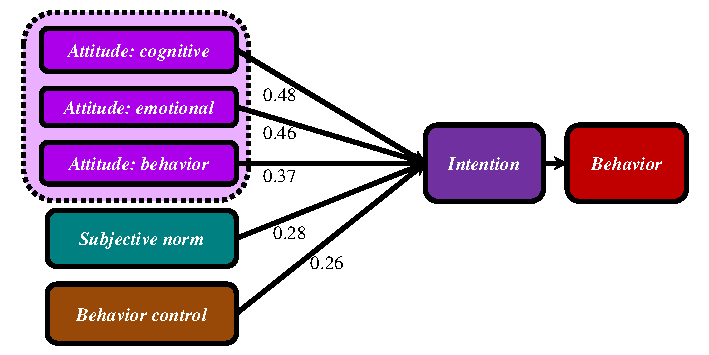
\includegraphics[width=9cm]{TpbTopH.pdf}
   \caption[Fig_AggregModel]{Aggregated  model of genre selection.}
   \label{Fig_AggregModel}
 \end{center}
 \end{figure}


%\begin{table}[!h]
%  \centering
%   \begin{tabular}{|l|c|c|c|c|c|c|c|c|c|c|c|c|c|c|c|c|}
\hline
&\textbf{$\beta_{0}$}&\textbf{$\beta_{1}$}&\textbf{$\beta_{2}$}&\textbf{$\beta_{3}$}&\textbf{$\beta_{4}$}&\textbf{$\beta_{5}$}&\textbf{$\beta_{6}$}&\textbf{$\beta_{7}$}&\textbf{$\beta_{8}$}&\textbf{$\beta_{9}$}&\textbf{$\beta_{10}$}&\textbf{$\beta_{11}$}&\textbf{$\beta_{12}$}&\textbf{$\beta_{13}$}&\textbf{$\beta_{14}$}&\textbf{$\beta_{15}$}\\\hline
\textbf{Drama}&0.07&0.25&0.01&-0.02&0.30&0.00&0.04&0.42&0.04&-0.03&0.68&-0.05&-0.02&0.58&-0.05&0.00\\\hline
\textbf{Action}&-1.20&-0.05&0.08&0.63&0.07&0.44&-0.44&-1.51&0.98&-0.21&3.67&0.63&-0.57&-0.76&-0.62&0.35\\\hline
\textbf{Comedy}&1.48&0.17&-0.61&1.10&1.33&-0.18&-0.03&-6.49&1.23&-0.11&3.54&0.20&-0.32&0.43&-1.53&0.93\\\hline
\end{tabular}

%  \caption{Multivariate regression coefficients of linear model's scores as predictors, $R^2 = 0.89$.}
%  \label{Tab_top_MvRegress}
%\end{table}


%\begin{table}[!h]
%  \centering
%   \begin{tabular}{|l|c|c|c|c|c|c|c|c|c|c|c|c|c|c|c|}
\hline
&\textbf{$w_{1}$}&\textbf{$w_{2}$}&\textbf{$w_{3}$}&\textbf{$w_{4}$}&\textbf{$w_{5}$}&\textbf{$w_{6}$}&\textbf{$w_{7}$}&\textbf{$w_{8}$}&\textbf{$w_{9}$}&\textbf{$w_{10}$}&\textbf{$w_{11}$}&\textbf{$w_{12}$}&\textbf{$w_{13}$}&\textbf{$w_{14}$}&\textbf{$w_{15}$}\\\hline
\textbf{Drama/Action}&-347.15&-24.89&-3.97&25.46&-29.52&-19.47&269.96&-4.04&4.65&-50.01&-13.28&7.12&-66.53&-35.72&24.74\\\hline
\textbf{Drama/Comedy}&-453.31&-18.10&-8.46&-41.58&-21.18&-21.19&379.43&-5.92&6.46&-82.89&-12.99&6.19&-8.76&-8.30&13.00\\\hline
\textbf{Action/Comedy}&-106.16&6.79&-4.49&-67.04&8.34&-1.73&109.46&-1.88&1.81&-32.88&0.30&-0.93&57.77&27.42&-11.74\\\hline
\end{tabular}

%  \caption{Linear discriminant coefficients of linear model's scores.}
%  \label{Tab_top_LDA}
%\end{table}

We do not list and interpret the coefficients of MVR and LDA for the aggregated model here. We summarize the whole model by a list of explained variances and Fisher separabilities at Tab. \ref{Tab_all_R2andSeps}. All listed $R^2$ values including the aggregated $R^2=0.89$ are statistically significant and they indicate the relative weight of each sub-model in movie selection regarding genre. Behavior control contributed the least and the cognitive aspect of attributes contributed the most to the whole model. 

\begin{table}[!h]
  \centering
   \begin{tabular}{|l|c|c|c|c|c|}
\hline
&\textbf{Attr: cog.}&\textbf{Attr: emot.}&\textbf{Attr: behav.}&\textbf{Norms}&\textbf{Cont.}\\\hline\hline
$\textbf{R}^2$&0.49&0.46&0.37&0.28&0.26\\\hline
\textbf{Separability}&0.81&1.03&0.60&0.44&0.50\\\hline
\end{tabular}

  \caption{Proportion of the Explained variance $R^2$ and Fisher separability for the aggregated model.}
  \label{Tab_all_R2andSeps}
\end{table}



% - hierarchy
% - model selection


% - rezultate regresij: primarnih + scori
% - rezultate diskriminantne analize
 




\section{Discussion}\label{Sec_Disc}

The main goal of this paper was to introduce the theory of planned behavior into a user modeling;  the results suggested that introduction of TPB is likely to increase accuracy of RS. Below, we discuss most relevant issues regarding advantages, limitations, and further development RS backing with psychology based research. 

\vspace{0.6em}
\noindent{\bf What are the benefits of implementing TPB in user modeling?} One of the main reasons of the application of TPB in a given domain to further extend the understanding of underlying mechanisms that governs the way how users make their decisions. In the field of user modeling, these understanding relates to two aspects. The first one is understanding user adaptation as whole (for example, what are relevant factors in movie item selection) and can be summarized from the results of prediction model fitting. The second one is how the individual user's mechanism (what are individual factors in these selections foe a given user) and we explain it from individual users responses to the survey questions together with model fitting results. 

In the movie genre selection example presented in this research, we selected MVR \cite{CohenCohenWestAiken200208} and Linear discriminant analysis \cite{RencherChristensen201207}. The magnitude and the sign of regression coefficients of the fitted model are used tho explain the relationship between  the aspect addressed with this question (for example How important is peer opinion for you?). Large magnitude indicates stronger relationship and the sign indicates the direction of the relationship. This is the explanation of the movie selection process as whole. The explanation of individual users behavior is based on his individual answers. If the magnitude of regression coefficient for a given question is large and this user's answer assigns high importance to it, then this aspect has a relevant impact in his movie decision making. 

As seen from the previous paragraph reasoning, the explanation of TPB model is highly dependent on the selected prediction model (MVR in our case). This means that models of little or no explanation power (black boxes) are of less interest in TPB event if they could be applied and they would gain higher prediction accuracy. 

\vspace{0.6em}
\noindent{\bf When the TPB is applicable?}  For the statistical and machine learning reasons, the first requirement of for the successful application of TPB is the predefined behaviors are separable by the selected model. In our case, genres that are not separable by users attributes, norms and beliefs cannot be well modeled and  the fitted model would provide misleading results. 

The separability of modeled behaviors also limits the number of these behaviors. It is clear that in practice several hundred or thousands of behaviors cannot separable (user data acquisition would not tolerate it in the first place). This leads to an important limitation of TPB in user modeling meaning that the treatment individual items cannot be defined as a behavior but these items must be grouped in a smaller number of groups or the definition of behaviors is based on a completely different aspect of user adaptation. For example, a predefined behavior can be a specific user behavior pattern while interacting with the system that is relevant for the whole process of user adaptation. 

\vspace{0.6em}
\noindent{\bf What are options to integrate TPB models into RS?} The role and integration of TPB into a user adaptation procedures is mainly determined by the definition of behaviors. As already indicated, user actions related to individual content items as behaviors is not a good choice. 


\vspace{0.6em}
\noindent{\bf What are the issues of TPB user data acquisition?} The theory and practice of TPB shows that the surveys required to fit the TPB model accurately  enough are relatively long and they also demand a considerable effort of the respondent (end user) to provide relevant answers. In the context of user modeling, this means that the user data acquisition is relatively intrusive. On the other hand, since users'  attributes, norms and beliefs are changing very slowly time it is enough for the user to fill the survey once a year only. However, the sampling period may vary significantly according to the domain and also according to an individual user's practice. In our example,  attributes, norms and beliefs toward movie genre selection may change faster for those users who sees more films in given amount of time. 


\vspace{0.6em}
\noindent{\bf Does TPB allows cross-domain user modeling?} Cross-domain of user adaptation techniques are of great interest. The question is can TPB models, in particular Ajzen model assure cross-domain capabilities in terms that the attributes, norms and beliefs of the end user estimated in one domain (for example movie selection) are at least in part valid for the other domain (for example tourist destination selection). Unfortunately, in general the answer is no. The reason for this is simply the fact that she survey used to estimate these attributes, norms and beliefs must be very specifically related to the domain of behaviors. For instance, the relevance of certain factors is asked for movies or for tourist destinations and not about some general user opinion common to both domains. However, the research on life - styles \cite{Stadtmueller2013} \cite{Dewberry2013} indicates that there are strong relations among human behaviors in different domains. 

\vspace{0.6em}
\noindent{\bf What are crucial decisions in TPB model selection and fitting?} As outlined in Subsec. \ref{Sec_AzenProc}, the whole procedure is highly dependent on the selected behavior. The next decision is, according to the domain knowledge, what are relevant factors of user's beliefs about the behavior. After these factors are identified, the questionnaire can be designed and tested on a pilot set of users. A selection of prediction model follows where and the candidate models are evaluated on a pilot study. This selection also depends on the aim of the application of TPB model which is from busting the performance of user adaptation procedure to the explanation of the adaptation process itself. 

\vspace{0.6em}
\noindent{\bf What are benefits of using TPB as user modeling techniques?} After the above listed considerations one could argue what are the benefits of the introduction of TPB that are not available from advanced statistics and machine learning algorithms. We see the following benefits of TPB in user modeling domain:
\begin{enumerate}
 \item {\it Explanation of underlying mechanisms.} Deeper understanding of processes accompanying user adaptation usually lead to more effective adaptation procedures, more appropriate evaluation measures and procedures and fresh ideas of how to implement the user adaptation results for end users;
 \item {\it Guidelines for analyzed classes (called behaviors in TPB) definition.} The theory of TPB together with the domain knowledge allows the description and definition of behaviors that are decisive for the whole user adaptation process. The ability of TPB to take into account the adaptation domain specifics is of crucial importance here since the later development of user adaptation techniques showed that the effective adaptation as well as its performance evaluation is very much domain specific;
 \item {\it Guidelines for survey questions formulations.} According to the previous point reasoning, the TPB further provides explicit guidelines for user data acquisition survey construction. It is important to note that there is a large number of data driven studies in several domains that supports the theory of TPB and the description of behavioral, normative and control beliefs. This allows to construct more effective surveys resulting in more accurate user data at the same level of intrusion; 
 \item {\it The study of cross-domain user adaptation.} Cross-domain user adaptation is one way to reduce the intrusion of user data acquisition and to design more effective user adaptation techniques. As already indicated, no cross-domain of estimated beliefs in TPB is guarantied. However, the studies related to life styles \cite{Dewberry2013} shows the potential to link the correlated user behavior patterns in the way that allows to make conclusions of end user beliefs from original to correlated domain. This is related to our future work plans. 
\end{enumerate}

\section{Conclusion and further work}\label{Sec_ConcAndFW}

The work present in this paper aims at establishing the relevance of psychological human decision modeling theory of planned behavior (TPB) into the field of user modeling. The study contributes to the models applicable in user modeling, in particular to the explanation of these models. 

Our results show that the application of TPB in the area of recommender systems allows further insight into the underlying process of user's decision making, i.e. into factors that affect these decisions. These insights can be used to address several issues such as effective user data acquisition, understanding and mitigating reasons for unacceptable recommendations etc. As an important part of this research performed by an interdisciplinary team including engineers, mathematicians, and psychologists are the guidelines for the future applications of TPB in different areas of user modeling. They include behavior selection, user questionnaire construction, criteria variable construction, regression model selection and fitting, and the explanation of obtained results. 

Despite limitations of the proposed modeling, our study showed that such modeling improves the understanding of user adaptation process. It is not meant as a replacement of existing user modeling models (for example Matrix factorization in movie recommendations) but as a predictor of end user behaviors that affects the whole process. Such behaviors the selection of the device he use to consume the recommended service etc. Furthermore, in the discussion section we addressed several issues relevant for the application of TPB into the user modeling domain. 


% 
% 
% 
% \begin{figure}[h!]
% \begin{center}
%   \includegraphics[trim = 2cm 8cm 2cm 6cm, clip,width=\columnwidth]{valence.pdf}
%   \caption[labelInTOC]{figureCaption}
%   \label{fig:valence}
% \end{center}
% \end{figure}


%\usepackage{graphics} is needed for \includegraphics
%\begin{figure}[h!]
%\begin{center}
 % \includegraphics[trim = 2cm 1cm 2cm 1cm, clip,width=\columnwidth]{graphicalabstract.pdf}
 % \caption[labelInTOC]{Overview of the paper: from the rating matrix we calculated the users' and items' latent factors. Then we analyzed the affective properties of items and the personality properties of users that lie at the extremes of the first two latent factors.}
 % \label{fig:graphical_abstract}
%\end{center}
%\end{figure}



\bibliographystyle{splncs03}
\bibliography{rs_allbib}

\end{document}


% BUFFER

\subsection{OLD: Results: Behavior model}\label{SubSec_ResModelAnalyis}

In this subsection, we list and explain behaviour model coeficients for each subgroup of questions separatelly. 

\begin{table}[!h]
  \centering
   \begin{tabular}{|l|c|c|c|c|c|c|c|c|c|}
\hline
&\textbf{$\beta_{0}$}&\textbf{$\beta_{1}$}&\textbf{$\beta_{2}$}&\textbf{$\beta_{3}$}&\textbf{$\beta_{4}$}&\textbf{$\beta_{5}$}&\textbf{$\beta_{6}$}&\textbf{$\beta_{7}$}&\textbf{$\beta_{8}$}\\\hline
\textbf{Drama}&13.7&-0.9&-1.3&-0.3&-1.1&-0.1&0.6&-0.3&-0.2\\\hline
\textbf{Action}&-2.4&0.1&0.0&-0.0&0.2&0.3&-0.1&0.1&-0.0\\\hline
\textbf{Comedy}&-455.9&1.7&88.1&0.7&1.7&-0.3&-0.8&0.3&0.6\\\hline
\end{tabular}

  \caption{Logit regression coefficients of cognitive attitude toward the behaviour predictors}
  \label{Tab_attitudeCog_Logit}
\end{table}

\begin{table}[!h]
  \centering
   \begin{tabular}{|l|c|c|c|c|c|c|c|c|c|c|c|c|c|c|}
\hline
&\textbf{$\beta_{0}$}&\textbf{$\beta_{1}$}&\textbf{$\beta_{2}$}&\textbf{$\beta_{3}$}&\textbf{$\beta_{4}$}&\textbf{$\beta_{5}$}&\textbf{$\beta_{6}$}&\textbf{$\beta_{7}$}&\textbf{$\beta_{8}$}&\textbf{$\beta_{9}$}&\textbf{$\beta_{10}$}&\textbf{$\beta_{11}$}&\textbf{$\beta_{12}$}&\textbf{$\beta_{13}$}\\\hline
\textbf{Drama}&-80.1&-3.9&1.7&0.5&0.8&4.5&3.4&-0.5&0.6&3.2&6.6&-0.6&5.2&-0.3\\\hline
\textbf{Action}&56879.9&-79.9&-1838.8&3553.5&1060.4&-644.2&-1354.0&-287.0&5584.0&-1544.3&-9393.5&-4493.7&585.3&-4250.6\\\hline
\textbf{Comedy}&-232.9&20.8&37.0&-47.1&-8.9&-54.6&-82.6&-64.0&-17.3&1.7&91.4&72.7&34.3&23.1\\\hline
\end{tabular}

  \caption{Logit regression coefficients of emotive attitude toward the behaviour predictors}
  \label{Tab_attitudeEmot_Logit}
\end{table}

\begin{table}[!h]
  \centering
   \begin{tabular}{|l|c|c|c|c|c|c|c|c|c|c|c|c|c|c|}
\hline
&\textbf{$\beta_{0}$}&\textbf{$\beta_{1}$}&\textbf{$\beta_{2}$}&\textbf{$\beta_{3}$}&\textbf{$\beta_{4}$}&\textbf{$\beta_{5}$}&\textbf{$\beta_{6}$}&\textbf{$\beta_{7}$}&\textbf{$\beta_{8}$}&\textbf{$\beta_{9}$}&\textbf{$\beta_{10}$}&\textbf{$\beta_{11}$}&\textbf{$\beta_{12}$}&\textbf{$\beta_{13}$}\\\hline
\textbf{Drama}&791.2&-0.5&-11.6&-3.9&4.1&22.7&-1.1&2.4&37.5&-38.8&68.0&-289.9&-35.9&-6.2\\\hline
\textbf{Action}&-598.7&-0.9&8.7&3.3&1.7&-20.4&-1.5&-0.5&-47.6&53.5&-255.0&273.5&68.5&-35.0\\\hline
\textbf{Comedy}&-257.6&-0.7&1.4&3.1&-2.3&-7.1&3.3&1.7&27.0&37.3&32.8&-4.7&-56.1&39.5\\\hline
\end{tabular}

  \caption{Logit regression coefficients of behavioral attitude toward the behaviour predictors, part one}
  \label{Tab_attitudeBehA_Logit}
\end{table}

\begin{table}[!h]
  \centering
   \begin{tabular}{|l|c|c|c|c|c|c|c|c|c|c|c|c|c|}
\hline
&\textbf{$\beta_{0}$}&\textbf{$\beta_{1}$}&\textbf{$\beta_{2}$}&\textbf{$\beta_{3}$}&\textbf{$\beta_{4}$}&\textbf{$\beta_{5}$}&\textbf{$\beta_{6}$}&\textbf{$\beta_{7}$}&\textbf{$\beta_{8}$}&\textbf{$\beta_{9}$}&\textbf{$\beta_{10}$}&\textbf{$\beta_{11}$}&\textbf{$\beta_{12}$}\\\hline
\textbf{Drama}&0.0&-1.1&19.1&-139.6&2.1&2.3&-139.0&1.6&3.5&137.3&46.1&142.0&-1.9\\\hline
\textbf{Action}&0.0&-0.4&5.3&1.9&-4.1&-3.1&0.7&-0.1&-3.4&1.1&1.3&-4.7&1.1\\\hline
\textbf{Comedy}&0.0&308.9&-1192.8&203.2&455.9&107.0&238.5&-500.2&-95.0&165.1&58.9&295.1&24.7\\\hline
\end{tabular}

  \caption{Logit regression coefficients of behavioral attitude toward the behaviour predictors, part two}
  \label{Tab_attitudeBehB_Logit}
\end{table}

%\begin{table}[!h]
%  \centering
%   \begin{tabular}{|l|c|c|c|c|c|c|c|c|c|c|c|c|c|c|}
\hline
&\textbf{$\beta_{0}$}&\textbf{$\beta_{1}$}&\textbf{$\beta_{2}$}&\textbf{$\beta_{3}$}&\textbf{$\beta_{4}$}&\textbf{$\beta_{5}$}&\textbf{$\beta_{6}$}&\textbf{$\beta_{7}$}&\textbf{$\beta_{8}$}&\textbf{$\beta_{9}$}&\textbf{$\beta_{10}$}&\textbf{$\beta_{11}$}&\textbf{$\beta_{12}$}&\textbf{$\beta_{13}$}\\\hline
\textbf{Drama}&-80.1&-3.9&1.7&0.5&0.8&4.5&3.4&-0.5&0.6&3.2&6.6&-0.6&5.2&-0.3\\\hline
\textbf{Action}&56879.9&-79.9&-1838.8&3553.5&1060.4&-644.2&-1354.0&-287.0&5584.0&-1544.3&-9393.5&-4493.7&585.3&-4250.6\\\hline
\textbf{Comedy}&-232.9&20.8&37.0&-47.1&-8.9&-54.6&-82.6&-64.0&-17.3&1.7&91.4&72.7&34.3&23.1\\\hline
\end{tabular}

%  \caption{Logit regression coefficients of emotive attitude toward the behaviour predictors}
%  \label{Tab_attitudeEmot_Logit}
%\end{table}

\begin{table}[!h]
  \centering
   \begin{tabular}{|l|c|c|c|c|c|c|c|c|}
\hline
&\textbf{$\beta_{0}$}&\textbf{$\beta_{1}$}&\textbf{$\beta_{2}$}&\textbf{$\beta_{3}$}&\textbf{$\beta_{4}$}&\textbf{$\beta_{5}$}&\textbf{$\beta_{6}$}&\textbf{$\beta_{7}$}\\\hline
\textbf{Drama}&15.2&2.9&0.0&2.5&-1.4&2.1&-5.4&-4.8\\\hline
\textbf{Action}&-4.2&-1.1&0.4&-1.0&0.9&-1.6&1.9&1.5\\\hline
\textbf{Comedy}&-5.4&-10.2&-2.9&2.4&-1.3&10.2&-5.2&7.7\\\hline
\end{tabular}

  \caption{Logit regression coefficients of emotive attitude toward the behaviour predictors}
  \label{Tab_control_Logit}
\end{table}


%
%\subsubsection{Recommender system models and algorithms}
%
%Colaborative, content-based, hybrid
%
%% http://www.cs.carleton.edu/cs_comps/0607/recommend/recommender/algorithms.html  - literature below
%
%% http://www.slideshare.net/xlvector/recommender-system-algorithm-and-architecture-13098396
%
%A comprehensive presentation of various aspects of recommender systems are given in \cite{Konstan2012}. 
%
%A very popular and well studied RS algorithm is matrix factorization \cite{koren2009matrix}.   
%
%Several known procedures and algorithms form the field of Machine learning \cite{} and multivariate statistics are used in RS. 
%
%
%\subsubsection{Multimedia items recommendation systems}



%\subsection{Results: Factor analysis}\label{SubSec_ResFacAnalyis}
%
%\begin{table}[!h]
%  \centering
%   \begin{tabular}{|l|c|c|c|c|}
\hline
&\textbf{$F_{1}$}&\textbf{$F_{2}$}&\textbf{$F_{3}$}&\textbf{$F_{4}$}\\\hline
\textbf{$Q_{1}$}&0.95&0.02&-0.25&-0.15\\\hline
\textbf{$Q_{2}$}&0.10&-0.72&-0.07&0.18\\\hline
\textbf{$Q_{3}$}&-0.04&0.41&-0.47&-0.01\\\hline
\textbf{$Q_{4}$}&-0.08&0.17&0.62&-0.13\\\hline
\textbf{$Q_{5}$}&-0.32&0.12&0.12&-0.43\\\hline
\textbf{$Q_{6}$}&0.50&0.12&0.24&0.25\\\hline
\textbf{$Q_{7}$}&0.22&0.75&0.06&0.11\\\hline
\textbf{$Q_{8}$}&-0.06&0.01&-0.04&0.61\\\hline
\end{tabular}

%  \caption{Factor matrix of cognitive attitude toward the behaviour predictors}
%  \label{Tab_attitudeCog_FactorAn}
%\end{table}
%
%\begin{table}[!h]
%  \centering
%   \begin{tabular}{|l|c|c|c|c|}
\hline
&\textbf{$F_{1}$}&\textbf{$F_{2}$}&\textbf{$F_{3}$}&\textbf{$F_{4}$}\\\hline
\textbf{$Q_{1}$}&-0.06&0.69&0.11&-0.02\\\hline
\textbf{$Q_{2}$}&-0.13&-0.34&0.12&-0.14\\\hline
\textbf{$Q_{3}$}&0.15&0.37&-0.05&0.16\\\hline
\textbf{$Q_{4}$}&-0.03&0.02&0.78&-0.30\\\hline
\textbf{$Q_{5}$}&0.08&0.16&0.22&-0.41\\\hline
\textbf{$Q_{6}$}&-0.56&0.22&-0.67&-0.08\\\hline
\textbf{$Q_{7}$}&0.13&0.35&-0.03&0.00\\\hline
\textbf{$Q_{8}$}&-0.66&0.37&-0.36&0.39\\\hline
\textbf{$Q_{9}$}&0.40&0.47&0.07&-0.13\\\hline
\textbf{$Q_{10}$}&-0.26&0.52&-0.06&0.81\\\hline
\textbf{$Q_{11}$}&-0.22&0.71&-0.07&-0.07\\\hline
\textbf{$Q_{12}$}&0.97&0.18&-0.04&-0.13\\\hline
\textbf{$Q_{13}$}&0.61&0.14&0.06&-0.03\\\hline
\end{tabular}

%  \caption{Factor matrix of cognitive attitude toward the behaviour predictors}
%  \label{Tab_attitudeEmot_FactorAn}
%\end{table}
%
%%\begin{table}[!h]
%%  \centering
%%   \begin{tabular}{|l|c|c|c|c|}
\hline
&\textbf{$F_{1}$}&\textbf{$F_{2}$}&\textbf{$F_{3}$}&\textbf{$F_{4}$}\\\hline
\textbf{$Q_{1}$}&0.70&0.53&-0.13&0.29\\\hline
\textbf{$Q_{2}$}&0.99&0.13&-0.07&-0.04\\\hline
\textbf{$Q_{3}$}&0.05&0.61&0.27&0.23\\\hline
\textbf{$Q_{4}$}&0.43&0.28&-0.00&0.74\\\hline
\textbf{$Q_{5}$}&-0.04&0.98&0.18&-0.08\\\hline
\textbf{$Q_{6}$}&0.68&0.41&-0.14&0.44\\\hline
\textbf{$Q_{7}$}&0.18&0.69&-0.04&-0.05\\\hline
\textbf{$Q_{8}$}&-0.02&0.20&0.98&0.00\\\hline
\textbf{$Q_{9}$}&-0.09&-0.08&0.01&0.38\\\hline
\textbf{$Q_{10}$}&0.63&-0.27&0.23&-0.18\\\hline
\end{tabular}

%%  \caption{Factor matrix of cognitive attitude toward the behaviour predictors}
%%  \label{Tab_attitudeBeh_FactorAn}
%%\end{table}
%
%%\begin{table}[!h]
%%  \centering
%%   \input{Code/norms_FactorAn.tex}
%%  \caption{Factor matrix of cognitive attitude toward the behaviour predictors}
%%  \label{Tab_FactorAn}
%%\end{table}
%
%\begin{table}[!h]
%  \centering
%   \begin{tabular}{|l|c|c|c|}
\hline
&\textbf{$F_{1}$}&\textbf{$F_{2}$}&\textbf{$F_{3}$}\\\hline
\textbf{$Q_{1}$}&-0.73&0.20&0.33\\\hline
\textbf{$Q_{2}$}&0.09&0.98&-0.13\\\hline
\textbf{$Q_{3}$}&0.10&0.45&0.22\\\hline
\textbf{$Q_{4}$}&0.14&0.11&0.50\\\hline
\textbf{$Q_{5}$}&0.67&0.34&0.36\\\hline
\textbf{$Q_{6}$}&0.69&0.28&0.05\\\hline
\textbf{$Q_{7}$}&-0.20&-0.05&0.71\\\hline
\end{tabular}

%  \caption{Factor matrix of cognitive attitude toward the behaviour predictors}
%  \label{Tab_control_FactorAn}
%\end{table}


%=====================
%
%\subsection{Testing models}\label{SubSec_TestModels}
%
%As indicated in previous subsection, we report the modeling of each beliefs separately and the hierarchical model where scores regressed from beliefs were used as predictor variables. For each model we report selected regression coefficients when necessary for the interpretation, variance explained ($R^2$), selected linear discriminant coefficients and separability in terms of Fisher discriminant analysis \cite{RencherChristensen201207}.
%
%\subsubsection{Attribute toward the behavior: cognitive}\label{SubSec_Res_AttrCog}
%
%
%
%
%
%\subsubsection{Attribute toward the behavior: emotions}\label{SubSec_Res_AttrEmot}
%
%
%\begin{table}[!h]
%  \centering
%   \begin{tabular}{|l|c|c|c|c|c|c|c|c|c|c|c|c|c|c|}
\hline
&\textbf{$\beta_{0}$}&\textbf{$\beta_{1}$}&\textbf{$\beta_{2}$}&\textbf{$\beta_{3}$}&\textbf{$\beta_{4}$}&\textbf{$\beta_{5}$}&\textbf{$\beta_{6}$}&\textbf{$\beta_{7}$}&\textbf{$\beta_{8}$}&\textbf{$\beta_{9}$}&\textbf{$\beta_{10}$}&\textbf{$\beta_{11}$}&\textbf{$\beta_{12}$}&\textbf{$\beta_{13}$}\\\hline
\textbf{Drama}&0.15&0.01&0.00&-0.01&-0.01&0.01&-0.00&0.02&0.02&-0.01&-0.02&-0.02&-0.01&0.02\\\hline
\textbf{Action}&4.10&-0.03&0.06&-0.00&-0.05&0.25&-0.13&0.10&0.01&0.09&0.06&-0.26&-0.08&-0.18\\\hline
\textbf{Comedy}&4.31&0.05&0.09&-0.01&-0.02&-0.11&0.05&0.21&-0.15&-0.16&0.01&-0.05&-0.26&0.17\\\hline
\end{tabular}

%  \caption{Multivariate regression coefficients of emotive attitude toward the behavior predictors, $R^2 = 0.46$.}
%  \label{Tab_attitudeEmot_MvRegress}
%\end{table}
%
%
%\begin{table}[!h]
%  \centering
%   \begin{tabular}{|l|c|c|c|c|c|c|c|c|c|c|c|c|c|}
\hline
&\textbf{$w_{1}$}&\textbf{$w_{2}$}&\textbf{$w_{3}$}&\textbf{$w_{4}$}&\textbf{$w_{5}$}&\textbf{$w_{6}$}&\textbf{$w_{7}$}&\textbf{$w_{8}$}&\textbf{$w_{9}$}&\textbf{$w_{10}$}&\textbf{$w_{11}$}&\textbf{$w_{12}$}&\textbf{$w_{13}$}\\\hline
\textbf{Drama/Action}&3.60&-3.29&0.82&3.39&-4.74&2.19&-1.33&-1.35&-2.95&3.42&3.08&0.82&2.10\\\hline
\textbf{Drama/Comedy}&-1.30&1.41&0.60&0.17&2.03&0.84&-3.11&-5.94&3.44&9.22&3.39&0.01&-1.60\\\hline
\textbf{Action/Comedy}&-4.90&4.70&-0.22&-3.22&6.77&-1.35&-1.78&-4.59&6.40&5.80&0.31&-0.81&-3.70\\\hline
\end{tabular}

%  \caption{Linear discriminant coefficients of emotive attitude toward the behavior predictors.}
%  \label{Tab_attitudeEmot_LDA}
%\end{table}
%
%
%\subsubsection{Attribute toward the behavior: behavioral}\label{SubSec_Res_AttrBeh}
%
%
%
%\begin{table}[!h]
%  \centering
%   \begin{tabular}{|l|c|c|c|c|c|c|c|c|c|c|c|}
\hline
&\textbf{$\beta_{0}$}&\textbf{$\beta_{1}$}&\textbf{$\beta_{2}$}&\textbf{$\beta_{3}$}&\textbf{$\beta_{4}$}&\textbf{$\beta_{5}$}&\textbf{$\beta_{6}$}&\textbf{$\beta_{7}$}&\textbf{$\beta_{8}$}&\textbf{$\beta_{9}$}&\textbf{$\beta_{10}$}\\\hline
\textbf{Drama}&0.24&-0.00&0.00&-0.00&0.00&0.00&-0.00&0.00&-0.04&0.04&-0.01\\\hline
\textbf{Action}&3.55&0.01&-0.02&-0.01&-0.02&-0.01&0.00&0.00&0.04&0.23&-0.00\\\hline
\textbf{Comedy}&3.56&-0.00&-0.00&0.00&-0.00&-0.01&0.00&-0.00&-0.20&0.20&0.21\\\hline
\end{tabular}

%  \caption{Multivariate regression coefficients of behavioral attitude toward the behavior predictors, $R^2 = 0.37$.}
%  \label{Tab_attitudeBehA_MvRegress}
%\end{table}
%
%\begin{table}[!h]
%  \centering
%   \begin{tabular}{|l|c|c|c|c|c|c|c|c|c|c|}
\hline
&\textbf{$w_{1}$}&\textbf{$w_{2}$}&\textbf{$w_{3}$}&\textbf{$w_{4}$}&\textbf{$w_{5}$}&\textbf{$w_{6}$}&\textbf{$w_{7}$}&\textbf{$w_{8}$}&\textbf{$w_{9}$}&\textbf{$w_{10}$}\\\hline
\textbf{Drama/Action}&-0.07&0.15&0.13&0.31&0.29&-0.08&-0.13&-3.62&-2.66&0.50\\\hline
\textbf{Drama/Comedy}&-0.04&0.04&-0.07&0.02&0.13&0.04&0.05&0.91&2.29&-1.09\\\hline
\textbf{Action/Comedy}&0.03&-0.11&-0.20&-0.29&-0.15&0.12&0.18&4.53&4.95&-1.59\\\hline
\end{tabular}

%  \caption{Linear discriminant coefficients of behavioral attitude toward the behavior predictors.}
%  \label{Tab_attitudeBehA_LDA}
%\end{table}
%
%
%
%\subsubsection{Subjective norm}\label{SubSec_Res_Norms}
%
%\begin{table}[!h]
%  \centering
%   \begin{tabular}{|l|c|c|c|c|c|}
\hline
&\textbf{$\beta_{0}$}&\textbf{$\beta_{1}$}&\textbf{$\beta_{2}$}&\textbf{$\beta_{3}$}&\textbf{$\beta_{4}$}\\\hline
\textbf{Drama}&0.29&-0.01&-0.00&-0.02&-0.01\\\hline
\textbf{Action}&3.99&0.18&-0.19&0.02&-0.08\\\hline
\textbf{Comedy}&3.85&0.14&-0.03&-0.15&0.02\\\hline
\end{tabular}

%  \caption{Multivariate regression coefficients of subjective norm predictors, $R^2 = 0.28$.}
%  \label{Tab_norms_MvRegress}
%\end{table}
%
%\begin{table}[!h]
%  \centering
%   \begin{tabular}{|l|c|c|c|c|}
\hline
&\textbf{$w_{1}$}&\textbf{$w_{2}$}&\textbf{$w_{3}$}&\textbf{$w_{4}$}\\\hline
\textbf{Drama/Action}&-1.17&0.48&-0.08&1.69\\\hline
\textbf{Drama/Comedy}&-0.53&0.00&0.49&1.56\\\hline
\textbf{Action/Comedy}&0.64&-0.48&0.57&-0.13\\\hline
\end{tabular}

%  \caption{Linear discriminant coefficients of subjective norms predictors.}
%  \label{Tab_norms_LDA}
%\end{table}
%
%
%\subsubsection{Perceived behavioral control}\label{SubSec_Res_Control}
%
%
%\begin{table}[!h]
%  \centering
%   \begin{tabular}{|l|c|c|c|c|c|c|c|c|}
\hline
&\textbf{$\beta_{0}$}&\textbf{$\beta_{1}$}&\textbf{$\beta_{2}$}&\textbf{$\beta_{3}$}&\textbf{$\beta_{4}$}&\textbf{$\beta_{5}$}&\textbf{$\beta_{6}$}&\textbf{$\beta_{7}$}\\\hline
\textbf{Drama}&0.17&0.02&-0.02&0.02&0.01&0.01&-0.02&-0.02\\\hline
\textbf{Action}&3.85&0.01&-0.07&0.03&-0.03&0.06&0.02&-0.04\\\hline
\textbf{Comedy}&2.80&0.23&-0.22&-0.04&0.01&0.18&0.05&0.00\\\hline
\end{tabular}

%  \caption{Multivariate regression coefficients of emotive attitude toward the behavior predictors, $R^2 = 0.26$.}
%  \label{Tab_control_MvRegress}
%\end{table}
%
%\begin{table}[!h]
%  \centering
%   \begin{tabular}{|l|c|c|c|c|c|c|c|}
\hline
&\textbf{$w_{1}$}&\textbf{$w_{2}$}&\textbf{$w_{3}$}&\textbf{$w_{4}$}&\textbf{$w_{5}$}&\textbf{$w_{6}$}&\textbf{$w_{7}$}\\\hline
\textbf{Drama/Action}&0.04&0.40&-0.96&-0.00&-0.05&-0.22&0.86\\\hline
\textbf{Drama/Comedy}&-0.72&1.19&-0.05&-0.96&-0.22&-1.83&0.17\\\hline
\textbf{Action/Comedy}&-0.76&0.79&0.92&-0.96&-0.17&-1.61&-0.69\\\hline
\end{tabular}

%  \caption{Linear discriminant coefficients of emotive attitude toward the behavior predictors.}
%  \label{Tab_control_LDA}
%\end{table}
%
%
%\subsubsection{Hierarchical model}\label{SubSec_Res_HierarModel}
%


